%%%%%%%%%%%%%%%%%%%%%%%%%%%%%%%%%%%%%%%%%%%%%%%%%%%%%%%%%%%%%%%%%%%%%%
%%  Copyright by Wenliang Du.                                       %%
%%  This work is licensed under the Creative Commons                %%
%%  Attribution-NonCommercial-ShareAlike 4.0 International License. %%
%%  To view a copy of this license, visit                           %%
%%  http://creativecommons.org/licenses/by-nc-sa/4.0/.              %%
%%%%%%%%%%%%%%%%%%%%%%%%%%%%%%%%%%%%%%%%%%%%%%%%%%%%%%%%%%%%%%%%%%%%%%

\newcommand{\commonfolder}{../../common-files}

\documentclass[11pt]{article}

\usepackage[most]{tcolorbox}
\usepackage{times}
\usepackage{epsf}
\usepackage{epsfig}
\usepackage{amsmath, alltt, amssymb, xspace}
\usepackage{wrapfig}
\usepackage{fancyhdr}
\usepackage{url}
\usepackage{verbatim}
\usepackage{fancyvrb}
\usepackage{adjustbox}
\usepackage{listings}
\usepackage{color}
\usepackage{subfigure}
\usepackage{cite}
\usepackage{sidecap}
\usepackage{pifont}
\usepackage{mdframed}
\usepackage{textcomp}
\usepackage{enumitem}
\usepackage{hyperref}


% Horizontal alignment
\topmargin      -0.50in  % distance to headers
\oddsidemargin  0.0in
\evensidemargin 0.0in
\textwidth      6.5in
\textheight     8.9in 

\newcommand{\todo}[1]{
\vspace{0.1in}
\fbox{\parbox{6in}{TODO: #1}}
\vspace{0.1in}
}


\newcommand{\unix}{{\tt Unix}\xspace}
\newcommand{\linux}{{\tt Linux}\xspace}
\newcommand{\minix}{{\tt Minix}\xspace}
\newcommand{\ubuntu}{{\tt Ubuntu}\xspace}
\newcommand{\setuid}{{\tt Set-UID}\xspace}
\newcommand{\openssl} {\texttt{openssl}}

% Arrows
\newcommand{\pointleft}[1]{\reflectbox{\ding{217}} \textbf{\texttt{#1}}}
\newcommand{\pointright}[1]{\ding{217} \textbf{\texttt{#1}}}
\newcommand{\pointupleft}[1]{\reflectbox{\ding{218}} \textbf{\texttt{#1}}}

% Line numbers
\newcommand{\lineone}{\ding{192}\xspace}
\newcommand{\linetwo}{\ding{193}\xspace}
\newcommand{\linethree}{\ding{194}\xspace}
\newcommand{\linefour}{\ding{195}\xspace}
\newcommand{\linefive}{\ding{196}\xspace}
\newcommand{\linesix}{\ding{197}\xspace}
\newcommand{\lineseven}{\ding{198}\xspace}
\newcommand{\lineeight}{\ding{199}\xspace}
\newcommand{\linenine}{\ding{200}\xspace}


% Fancy headers
\pagestyle{fancy}
\lhead{\bfseries SEED Labs}
\chead{}
\rhead{\small \thepage}
\lfoot{}
\cfoot{}
\rfoot{}


\definecolor{dkgreen}{rgb}{0,0.6,0}
\definecolor{gray}{rgb}{0.5,0.5,0.5}
\definecolor{mauve}{rgb}{0.58,0,0.82}
\definecolor{lightgray}{gray}{0.90}


\lstset{%
  frame=none,
  language=,
  backgroundcolor=\color{lightgray},
  aboveskip=3mm,
  belowskip=3mm,
  showstringspaces=false,
%  columns=flexible,
  basicstyle={\small\ttfamily},
  numbers=none,
  numberstyle=\tiny\color{gray},
  keywordstyle=\color{blue},
  commentstyle=\color{dkgreen},
  stringstyle=\color{mauve},
  breaklines=true,
  breakatwhitespace=true,
  tabsize=3,
  columns=fullflexible,
  keepspaces=true,
  escapeinside={(*@}{@*)}
}

\newcommand{\newnote}[1]{
\vspace{0.1in}
\noindent
\fbox{\parbox{1.0\textwidth}{\textbf{Note:} #1}}
%\vspace{0.1in}
}


%% Submission
\newcommand{\seedsubmission}{You need to submit a detailed lab report, with screenshots,
to describe what you have done and what you have observed.
You also need to provide explanation
to the observations that are interesting or surprising.
Please also list the important code snippets followed by
explanation. Simply attaching code without any explanation will not
receive credits.}

%% Book
\newcommand{\seedbook}{\textit{Computer \& Internet Security: A Hands-on Approach}, 3rd
Edition, by Wenliang Du. See details at \url{https://www.handsonsecurity.net}.\xspace}

\newcommand{\seedisbook}{\textit{Internet Security: A Hands-on Approach}, 3rd
Edition, by Wenliang Du. See details at \url{https://www.handsonsecurity.net}.\xspace}

\newcommand{\seedcsbook}{\textit{Computer Security: A Hands-on Approach}, 3rd
Edition, by Wenliang Du. See details at \url{https://www.handsonsecurity.net}.\xspace}

\newcommand{\seedcibook}{\textit{Computer \& Internet Security: A Hands-on Approach}, 3rd
Edition, by Wenliang Du. See details at \url{https://www.handsonsecurity.net}.\xspace}

%% Videos
\newcommand{\seedisvideo}{\textit{Internet Security: A Hands-on Approach},
by Wenliang Du. See details at \url{https://www.handsonsecurity.net/video.html}.\xspace}

\newcommand{\seedcsvideo}{\textit{Computer Security: A Hands-on Approach},
by Wenliang Du. See details at \url{https://www.handsonsecurity.net/video.html}.\xspace}

%% Lab Environment
\newcommand{\seedenvironment}{This lab has been tested on our pre-built
Ubuntu 16.04 VM, which can be downloaded from the SEED website.\xspace}

\newcommand{\seedenvironmentA}{This lab has been tested on our pre-built
Ubuntu 16.04 VM, which can be downloaded from the SEED website.\xspace}

\newcommand{\seedenvironmentB}{This lab has been tested on our pre-built
Ubuntu 20.04 VM, which can be downloaded from the SEED website.\xspace}

\newcommand{\seedenvironmentC}{This lab has been tested on the SEED
Ubuntu 20.04 VM. You can download a pre-built image from the SEED website, 
and run the SEED VM on your own computer. However,
most of the SEED labs can be conducted on the cloud, and 
you can follow our instruction to create a SEED VM on the cloud.\xspace}

\newcommand{\seedenvironmentAB}{This lab has been tested on our pre-built
Ubuntu 16.04 and 20.04 VMs, which can be downloaded from the SEED website.\xspace}

\newcommand{\nodependency}{Since we use containers to set up the lab environment, 
this lab does not depend much on the SEED VM. You can do this lab
using other VMs, physical machines, or VMs on the cloud.\xspace}

\newcommand{\adddns}{You do need to add the required IP address mapping to
the \texttt{/etc/hosts} file.\xspace}






\newcommand{\seedlabcopyright}[1]{
\vspace{0.1in}
\fbox{\parbox{6in}{\small Copyright \copyright\ {#1}\ \ by Wenliang Du.\\
      This work is licensed under a Creative Commons
      Attribution-NonCommercial-ShareAlike 4.0 International License.
      If you remix, transform, or build upon the material, 
      this copyright notice must be left intact, or reproduced in a way that is reasonable to
      the medium in which the work is being re-published.}}
\vspace{0.1in}
}





\newcommand{\firewallFigs}{./Figs}
\lhead{\bfseries SEED Labs -- Firewall Evasion Lab}

\begin{document}



\begin{center}
{\LARGE Firewall Evasion Lab: Bypassing Firewalls using VPN}
\end{center}


\seedlabcopyright{2018}

\newcounter{task}
\setcounter{task}{1}
\newcommand{\tasks} {\bf {\noindent (\arabic{task})} \addtocounter{task}{1} \,}


% *******************************************
% SECTION
% ******************************************* 
\section{Overview}


Organizations, Internet Service Providers (ISPs), and countries often block
their internal users from accessing certain external sites. This is called
egress filtering. 
For example, to prevent work-time distraction, many companies set up their egress firewalls
to block social network sites, so their employee cannot access those sites
from inside their network. For political reasons, many countries set up egress filtering at their
ISPs to block their people from accessing
selected foreign websites. Unfortunately, these firewalls can be easily
bypassed, and services/products that help users bypass firewalls are widely
available on the Internet. The most commonly used technology to bypass
egress firewalls is Virtual Private Network (VPN).
In particular, this technology is widely used by smartphone users that are affected by
egress filtering; there are many VPN apps (for Android, iOS, and other
platforms) that can help users bypass egress firewalls. 


The learning objective of this lab is for students to see 
how VPN works in action and how VPN can help bypass egress firewalls.     
We will implement a very simple VPN in this lab, and use it to bypass
firewalls. A typical VPN depends on two pieces of technologies: IP tunneling
and encryption. The tunneling technology is the most essential one to help
bypass firewalls; the encryption technology is for protecting the content
of the traffic that goes through the VPN tunnel. 
For the sake of simplicity, we will only focus on the tunneling part,
so the traffic inside our tunnel is not encrypted. We have a separate
VPN lab, which covers both tunneling and encryption. If readers are
interested, they can work on our VPN lab to learn how to build a complete
VPN. In this lab, we only focus on how to use VPN tunnel to bypass firewalls.
This lab covers the following topics:

\begin{itemize}[noitemsep]
\item Firewall
\item VPN
\end{itemize}


\paragraph{Readings and videos.}
Detailed coverage of firewalls, firewall evasion techniques, and VPN can be found in
the following

\begin{itemize}
\item Chapters 17 and 19 of the SEED Book, \seedbook
\item Sections 8 and 9 of the SEED Lecture, \seedisvideo
\end{itemize}


\paragraph{Lab environment.} \seedenvironmentB
 


% *******************************************
% SECTION
% ******************************************* 
\section{Lab Tasks}




% -------------------------------------------
% SUBSECTION
% ------------------------------------------- 
\subsection{Task 1: VM Setup}

 
We need two machines, one inside the firewall, and the other
outside the firewall. The objective is to help the machine
inside the firewall to reach out to the external sites blocked by the firewall. 
We use two virtual machines, VM1 and VM2, for these two machines. 
VM1 and VM2 are supposed to be two machines connected via the Internet through
routers. This setup may require more than two VMs. 
For the sake of simplicity, we use a LAN to emulate the Internet connection.
Basically, we simply connect VM1 and VM2 to a LAN using the \texttt{NAT Network} 
adapter. Figure~\ref{vpn_firewall:fig:labsetup} depicts the lab setup.

\begin{figure}[htb]
  \begin{center}
    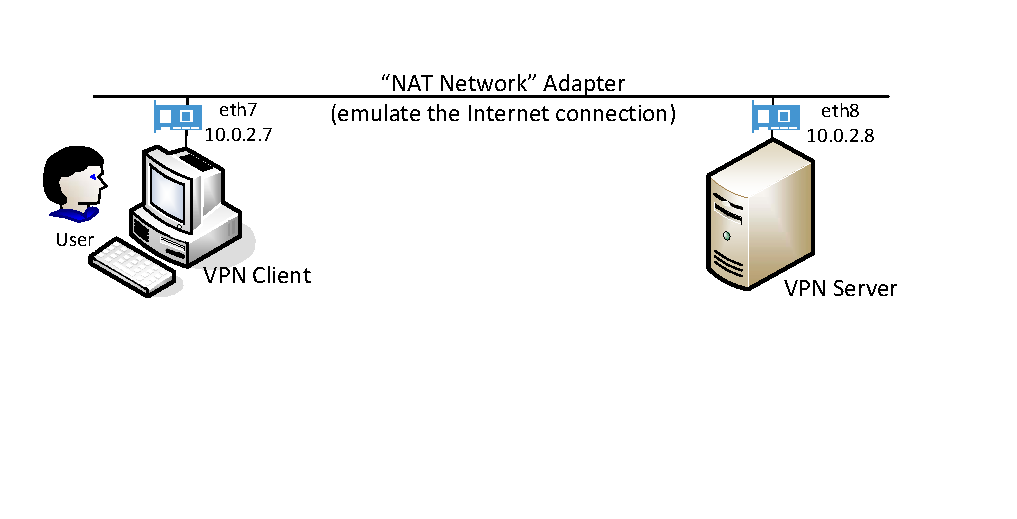
\includegraphics[width=0.9\textwidth]{\firewallFigs/Host2Gateway.pdf}
  \end{center}
  \caption{Lab Environment Setup}
  \label{vpn_firewall:fig:labsetup}
\end{figure}



% -------------------------------------------
% SUBSECTION
% ------------------------------------------- 
\subsection{Task 2: Set up Firewall}

In this task, you will set up a firewall on VM1 to block the access of a target website. You
need to make sure that the IP address of the target web site is either fixed or in a fixed
range; otherwise, you may have trouble completely blocking this website. Please refer to the
Firewall Lab for details about how to blocking websites.

In the real world, the firewall should run on a separate machine, not on VM1. To minimize the number of VMs
used in this lab, we put the firewall on VM1. Setting up the firewall on VM1 requires the superuser
privilege, and so does the setup of the VPN tunnel. One may immediately say that if we already
have the superuser privilege, why cannot we just simply disable the firewall on VM1. This is a good argument,
but keep in mind, we put the firewall on VM1 simply because we do not want to create another VM
in the lab environment. Therefore, although you have the superuser privilege on VM1, you are
not allowed to use the privilege to reconfigure the firewall. You have to use VPN to bypass
it.

Compared to putting the firewall on an external machine, putting the firewall on VM1 does have
a small issue that we need to deal with. When we set up the firewall to block packets, we need
to make sure not to block the packets from getting to the virtual interface used by the VPN, or even our
VPN will not be able to get the packets.  Therefore, we cannot set the firewall rule before the
routing, nor can we set the firewall rule on the virtual interface. We just need to set the
rule on VM1's real network interface, so it will not affect the packets that go to the virtual
interface. The following command blocks all traffic to \texttt{93.184.216.0/24} 
network (\texttt{example.com}). 

\begin{lstlisting}
$ sudo iptables -A OUTPUT -o enp0s3 -d 93.184.216.0/24 -j DROP
\end{lstlisting}

Please identify a website that you would like to block, set up the firewall,
and then demonstrate that your firewall is working and the target IP address is no longer 
reachable. Provide screenshots in your lab report.  


% -------------------------------------------
% SUBSECTION
% ------------------------------------------- 
\subsection{Task 3: Bypassing Firewall using VPN}



The idea of using VPN to bypass firewall is depicted in 
Figure~\ref{vpn_firewall:fig:bypassing}. 
We establish a VPN tunnel between VM1 (VPN Client VM) 
and VM2 (VPN Server VM). 
When a user on VM1 tries to access a blocked site, the traffic will not directly 
go through its network adapter, because it will be blocked. Instead, the 
packets to the blocked site from VM1 will be routed to the VPN tunnel and arrive at VM2. Once
they arrive there, VM2 will route them to the final destination. 
When the reply packets come back, it will come back to VM2, which will then redirect the
packets to the VPN tunnel, and eventually get the packet back to VM1. That is how the VPN helps
VM1 to bypass firewalls. 

\begin{figure}[htb]
\begin{center}
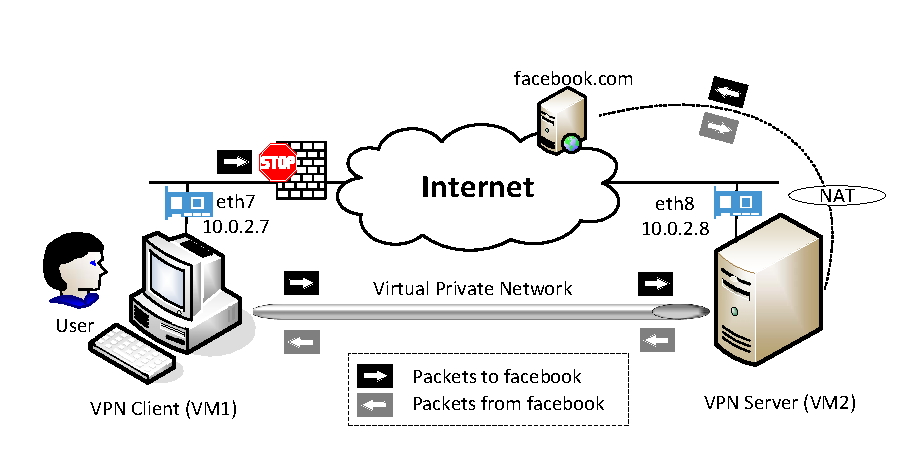
\includegraphics[width=1.0\textwidth]{\firewallFigs/BypassingFirewall.pdf}
\end{center}
\caption{Bypassing firewall using VPN}
\label{vpn_firewall:fig:bypassing}
\end{figure}
 


We have created a sample VPN program, including a client program (\texttt{vpnclient})  and
a server program (\texttt{vpnserver}), both of which can be downloaded from
this lab's web site. This simple VPN program only establishes a VPN tunnel 
between the client and server; it does not encrypt the tunnel traffic.
The program is explained in details in the SEED book (in the VPN chapter).


\begin{figure}[htb]
\begin{center}
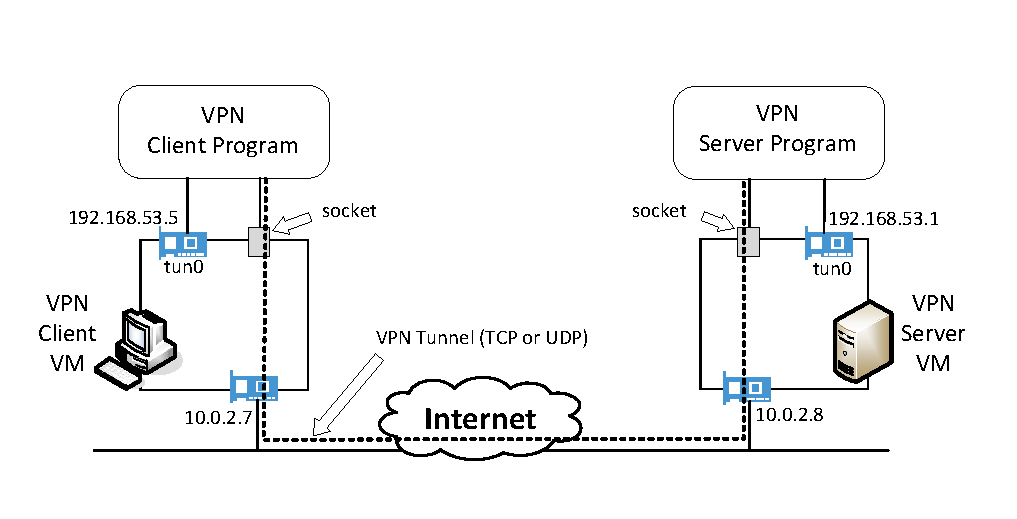
\includegraphics[width=0.9\textwidth]{\firewallFigs/ClientServerTunnel.pdf}
\end{center}
\caption{VPN client and server}
\label{vpn_firewall:fig:client_server}
\end{figure}

The \texttt{vpnclient} and \texttt{vpnserver} programs are the two ends of
a VPN tunnel. They communicate with each other using either TCP or UDP via the sockets
depicted in Figure~\ref{vpn_firewall:fig:client_server}. In our sample code, we choose
to use UDP for the sake of simplicity.  The dotted line between the
client and server depicts the path for the VPN tunnel.
The VPN client and server programs connect to the hosting system via a
TUN interface, through which they do two things: (1) get IP packets from
the hosting system, so the packets can be sent through the tunnel, (2) get IP packets from the
tunnel, and then forward it to the hosting system, which will forward the
packet to its final destination.
The following procedure describes how to create a VPN tunnel
using the \texttt{vpnclient} and \texttt{vpnserver} programs.


\paragraph{Step 1: Run VPN Server.}
We first run the VPN server program \texttt{vpnserver} on the Server VM.
After the program runs, a virtual TUN network interface will appear
in the system (we can see it using the \texttt{"ifconfig -a"} command; the name of the
interface will be \texttt{tun0} in most cases, but they can be
\texttt{tunX}, where \texttt{X} is a number).
This new interface is not yet configured, so we need to configure it by giving it an IP
address. We use \texttt{192.168.53.1} for this interface, but you can use 
other IP addresses. 


Run the following commands. The first command will start the server
program, and the second command assigns an IP address to the \texttt{tun0}
interface and then activates it. It should be noted that the first
command will block and wait for connections,
so we need to find another window run the second command.


\begin{lstlisting}
$ sudo ./vpnserver

Run the following command in another window:
$ sudo ifconfig tun0 192.168.53.1/24 up
\end{lstlisting}

Unless specifically configured, a computer will only act as a host,
not as a gateway. The VPN Server needs to forward packets to other destinations,
so it needs to function as a gateway. We need to
enable the IP forwarding for a computer to behave like a gateway.
IP forwarding can be enabled
using the following command:

\begin{lstlisting}
$ sudo sysctl net.ipv4.ip_forward=1
\end{lstlisting}



\paragraph{Step 2: Run VPN Client.} 
We now run the VPN client program on the Client
VM.  We run the following command on this machine (the first command
will connect to the VPN server program running on {\tt 10.0.2.8}.
This command will block as well, so we need to find another window to
configure the \texttt{tun0} interface created by the VPN client program.
We assign IP address \texttt{192.168.53.5} to the \texttt{tun0} interface~(you
can choose other IP addresses).


\begin{lstlisting}
On VPN Client VM:
$ sudo ./vpnclient 10.0.2.8

Run the following command in a different window
$ sudo ifconfig tun0 192.168.53.5/24 up
\end{lstlisting}



\paragraph{Step 3: Set Up Routing on Client and Server VMs.}
After the above two steps, the tunnel will be established.
Before we can use the tunnel, we need to set up routing
paths on both client and server machines to direct the intended traffic through
the tunnel. 
We can use the \texttt{route} command to add an routing entry. The
following example shows how to route the \texttt{10.20.30.0/24}-bound
packets to the interface \texttt{eth0}.

\begin{lstlisting}
$ sudo route add -net 10.20.30.0/24 eth0
\end{lstlisting}

To bypass firewalls on the Client VM, you need to set up 
routing entries accordingly, so the traffics to the blocked site
will be routed towards the VPN. You need to think about what 
routing entries to add in order to bypass the firewall. 



\paragraph{Step 4: Set Up NAT on Server VM.}
When the final destination sends packets back to users, the packet
will be sent to the VPN Server first (think about why and write down your answer 
in the report). The return packet will reach the VPN Server's NAT
adapter first (because the source IPs of all  the outgoing
packets from the Server VM are changed to the NAT's external IP address (which is basically the host computer's IP
address in our setup). Usually, the NAT will replace the destination IP address with the IP
address of the original packet (i.e. \texttt{192.168.53.5} in our case), and give it back to whoever owns
the IP address.  Unfortunately, we have a problem here.


Before the NAT sends out the packet, it needs to know the MAC address of the machine who owns
\texttt{192.168.53.5}, so it sends an ARP request. Our private network is virtual, and 
this IP address belongs to the \texttt{tun0} interface on the VPN Client.  
therefore, \texttt{192.168.53.5} will not receive the ARP request (even if it does, it has no
use). The NAT will then drop the packet, because the recipient does not exist.


The actual recipient should be the VPN Server VM, even though it does not own 
\texttt{192.168.53.5}.  If
we can configure the NAT as a gateway, we can ask the NAT to route the packets for
\texttt{192.168.53.5} to 
the VPN Server, which will eventually deliver the packets through the tunnel to the VPN Client. However,
we have not figured out how to configure the NAT as a gateway in VirtualBox, we did
come up two work-around solutions. One idea is to ``fool'' the NAT to believe that the MAC address of
\texttt{192.168.53.5} is the VPN Server VM's MAC address, so the packet will be delivered to
the VPN Server by the NAT. We can achieve this using an ARP cache poisoning on the NAT, basically telling the
NAT before hand about the MAC address of \texttt{192.168.53.5}.

A better solution to get round the limitation of the NAT is to create another NAT
right on the Server VM, so all packets coming out of the Server VM will have this VM's IP address as their source IP.
To reach the Internet, these packets will go through another NAT, which is provided by
VirtualBox, but since the source IP is the Server VM, this second NAT will have no problem relaying back
the returned packets from the Internet to the Server VM. Using this solution, we do not need to use ARP
cache poisoning to ``fool'' the NAT any more. The following commands can enable the NAT on
the Server VM~(in your case, the name of the \texttt{NAT Network} adapter may not be called 
\texttt{enp0s3}; you just need to find its real name on your VM):

    
\begin{lstlisting}
$ sudo iptables -t nat -A POSTROUTING -j MASQUERADE -o enp0s3
\end{lstlisting}
    


\paragraph{Demonstration.}
If you have done the steps above correctly, you should be able to bypass
the firewall. You should show that you can reach the blocked web site from Client VM
via the VPN.  Your solution should
not only work for web traffic, but also for all other traffic. For example, if the blocked
machine runs a \texttt{telnet} server, you should be able to \texttt{telnet} to this blocked server from
Client VM. 

In your lab report, you should provide the evidence to show that your traffic did go through
the VPN tunnel, not through some ``side doors''. The best way to show that is to capture the
network traffic using Wireshark, and describe the path of your packets using the captured
traffic. Without such an evidence, we have no idea whether your success is due to a
mis-configured firewall (i.e. the targeted web site is not blocked at all) or due to your VPN.



% *******************************************
% SECTION
% ******************************************* 
\section{Submission Requirement}

%%%%%%%%%%%%%%%%%%%%%%%%%%%%%%%%%%%%%%%%

You need to submit a detailed lab report, with screenshots,
to describe what you have done and what you have observed.
You also need to provide explanation
to the observations that are interesting or surprising.
Please also list the important code snippets followed by
explanation. Simply attaching code without any explanation will not
receive credits.

%%%%%%%%%%%%%%%%%%%%%%%%%%%%%%%%%%%%%%%%


\end{document}


